\documentclass[a4paper]{article}

\usepackage[12pt]{extsizes}

\usepackage[T2A]{fontenc}
\usepackage[utf8]{inputenc}

\usepackage[english,russian]{babel}

\usepackage{indentfirst}
\usepackage{scrextend}
\usepackage{fancyhdr}

\usepackage{xr}
\usepackage{verbatimbox}
\usepackage{caption}
\usepackage{graphicx}

\usepackage{listings}
\usepackage{color}
\definecolor{mygreen}{rgb}{0,0.6,0}
\definecolor{mygray}{rgb}{0.5,0.5,0.5}
\lstset{extendedchars=\true,
		breaklines=true,
		breakatwhitespace=true,
		captionpos=b,
		keepspaces=true,
		keywordstyle=\color{blue},
		numbers=left,
		tabsize=4,
		numberstyle=\tiny\color{mygray},
		commentstyle=\color{mygreen},
		language=C,
		basicstyle=\ttfamily,
		showstringspaces=false,
		title=\lstname
		}
 
\usepackage{geometry} % Меняем поля страницы
\geometry{left=2.8cm}% левое поле
\geometry{right=2.8cm}% правое поле
\geometry{top=2.5cm}% верхнее поле
\geometry{bottom=3cm}% нижнее поле

\usepackage{perpage}
\MakePerPage{footnote}

\setcounter{tocdepth}{2}
\ifx
Выставление глубины оглавления
n=4 это chapter, section, subsection, subsubsection и paragraph;
n=3 это chapter, section, subsection и subsubsection;
n=2 это chapter, section, и subsection;
n=1 это chapter и section;
n=0 это chapter.
\fi

\renewcommand*\thesection{\arabic{section}.}
\renewcommand{\thesubsection}{\thesection\arabic{subsection}}

\newcommand{\newpar}{\par\medskip}

\newcommand{\sbt}{
	\,\begin{picture}(-1,1)(-1,-3)\circle*{4}\end{picture}\ 
}
\newcommand{\sbti}{\sbt~~}

\newcommand{\linux}{Linux}
\newcommand{\linuxv}{\linux\ v.3.9.2\ }
\newcommand{\gnu}{GNU}
\newcommand{\gnulinux}{\gnu/\linux}
\newcommand{\archlinux}{Arch Linux}
\newcommand{\fulllinux}{\archlinux, ядро \linuxv}
\newcommand{\unix}{UNIX\ }

\newcommand{\linuxpath}[1]{\texttt{#1}}
\newcommand{\linuxutil}[1]{\texttt{#1}}
\newcommand{\linuxcommand}[1]{\texttt{#1}}
\newcommand{\src}[1]{\linuxcommand{#1}}
\newcommand{\key}[1]{\src{<#1>}}

\bibliographystyle{plain}

\begin{document}
	\thispagestyle{fancy}

\fancyhead[C]{
	Федеральное государственное бюджетное 
	образовательное учреждение высшего 
	профессионального образования\\
	<<Московский государственный технический 
	университет им.~Н.\,Э.~Баумана>>
}
\fancyfoot[C]{ Москва, 2013г. }

\vspace*{2cm}

\begin{flushright}
	\Large{ Факультет: }\\
	\large{ <<Информатика и системы управления>> }\\
	\Large{ Кафедра: }\\
	\large{ <<Программное обеспечение ЭВМ и\\ 
		информационные технологии>> }
\end{flushright}

\vspace{2cm}

\begin{LARGE} 
	\begin{center} 
		Расчетно\,--\,пояснительная записка\\
		к курсовому проекту\\ 
		\vspace{2cm}
		Разработка программного обеспечения, обеспечивающего ввод текста
		с помощью дополнительной цифровой клавиатуры в ОС
		\gnulinux 
	\end{center}
\end{LARGE}

\vspace{5cm}

\begin{flushright}
	\begin{tabular}{ll}
	Руководитель курсового проекта:&Рязанова~Н.\,Ю.\\
	Исполнитель курсового проекта:&Бережной~П.\,Ю.
	\end{tabular}
\end{flushright}

\newpage
\setcounter{page}{1}

	\tableofcontents
	\newpage
	\addcontentsline{toc}{section}{Введение}
\section*{Введение}

Клавиатура -- одно из самых важных переферийных устройств компьютера. Не смотря
на совершенствование в наше время таких устройств ввода как мыши, трекболы, тачпады,
тачскрины и многих других, клавиатура все же остается основным и самым удобным средством
ввода информации. 
\newpar
Очень часто возникает необходимость в переназначении клавиш на клавиатуре:
\begin{itemize}
	\item Стандартное расположение клавиш неудобно при работе
		с определенным программным обеспечением;
	\item При переходе с одного типа клавиатуры на другой трудно привыкнуть
		к новому расположению клавиш.
\end{itemize}
\newpar

Длительное использование клавиатуры часто приводит к западанию клавиш.
Для решения данной проблемы можно использовать дополнительные методы ввода,
например имитация цифровой клавиатуры телефона с помощью дополнительной цифровой клавиатуры 
компьютера.
\newpar

Под операционной системой \linux\ существуют стандартные средства и программы, 
которые частично выполняют поставленную задачу. 
Примером стандартных средств может служить задание собственной маски клавиш клавиатуры
в файле \linuxpath{/usr/share/kbd/keymaps/i386/qwerty/personal.map}\footnote{Действительно для %
дистрибутива \fulllinux} в любимом текстовом редакторе и задание полученой
кодировки в файле \linuxpath{/etc/vconsole.conf}\,\footnotemark[1].
Примером программ для переназначения функций клавиш клавиатуры может служить утилита
\linuxutil{xmodmap} из пакета \linuxutil{xorg-server-utils}\footnote{Подробнее, \linuxcommand{man xmodmap}}.\\
Средств для полной реализации поставленной задачи нет.
\newpage
	
	\section{Аналитический раздел}

\subsection{Постановка задачи}
В соответствии с техническим заданием на курсовой проект необходимо разработать
программное обеспечение, позволяющее использовать дополнительную цифровую клавиатуру
для ввода текста.
\begin{itemize}
	\item Программное обеспечение должно переопределять
		набор цифровых клавиш дополнительной клавиатуры;
	\item Программное обеспечение должно позволять вводить несколько
		различных символов при нажатии на одну и ту же клавишу дополнительной
		цифровой клавиатуры;
	\item Программное обеспечение должно учитывать число нажатий клавиши
		и время отсутствия нажатия;
	\item Программное обеспечение не должно нарушать или замедлять работу системы.
\end{itemize}

Поставленную задачу нельзя решить в адрессном пространстве пользователя.
Однако это можно сделать путем написания соответствующего драйвера.

\subsection{Подсистема ввода-вывода}
Подсистема ввода/вывода \linux\ обеспечивает простой и универсальный интерфейс 
для устройств, находящихся на плате. Подсистемой ввода/вывода 
поддерживаются три вида устройств:
\begin{itemize}
	\item Символьные устройства для поддержки последовательных устройств;
	\item Блочные устройства для поддержки устройств с произвольным доступом. 
		Блочные устройства имеют важное значение для реализации файловых систем;
	\item Сетевые устройства, которые поддерживают широкий спектр устройств на канальном уровне;
\end{itemize}

Клавиатура относится к классу символьных устройств, где данные передаются посимвольно.
\newpar

Управление работой клавиатуры в текстовом режиме осуществляется драйвером терминала, который входит в состав ядра \linux.
Драйвер терминала состоит из двух отдельных драйверов: драйвера клавиатуры и драйвера экрана. Драйвер
клавиатуры обрабатывает нажатия клавиш пользователем и передает результат прикладной программе, которая, в
свою очередь, посылает экранному драйверу символы которые должны быть отображены на экране.
При каждом нажатии на клавишу микропроцессор клавиатуры генерирует последовательность скан-кодов, которая представляет
собой набор из двух или больше числа байтов.
Эта последовательность передается драйверу клавиатуры, который может работать в одном из четырех режимов:

\begin{itemize}
	\item K\_ROW, когда прикладной программе передается последовательность скан-кодов, сгенерированных клавиатурой.
		Этот режим используется при работе с приложениями, которые имеют свой собственный драйвер клавиатуры. Примером
		такого приложения является система \linuxcommand{XWindow}.
	\item K\_MEDIUMRAW, когда скан-код клавишт преобразуется в один из 127 возможных кодов, называемых кодами клавиш (keycodes).
		Каждый код клавиши состоит из кода нажатия клавиши и кода отпускания клавиши. Преобразование скан-кодов
		в коды клавиш осуществляется в соответствии с внутренней таблицей драйвера клавиатуры. Обычно, 
		эта таблица фиксирована, и изменять ее не требуется, хотя в системе существуеткоманды \linuxcommand{getkeycodes} и 
		\linuxcommand{setkeycodes}, с помощью которых можно просмотреть или изменить некоторые соответствия в этой
		таблице. Эти команды используются только в том случае, если клавиатура программируемая.
	\item K\_XLATE (или режим ASCII), когда коды клавиши преобразуются в ASCII-код символа или в некоторую последовательность
		ASCII-кодов символов в соответствии с таблицей раскладки клавиатуры, которая хранится в виде отдельного файла.
		Например, для \fulllinux\ по умолчанию используется файл \linuxpath{defkeymap.map.gz} в 
		каталоге \linuxpath{/usr/share/\-kbd/\-keymaps/\-i386/qwerty}. Команда \linuxcommand{dumpkeys} выводит на экран
		содержание действующей в данный момент таблицы раскладки клавиатуры, а команда \linuxcommand{loadkeys} загружает
		в драйвер таблицу раскладки клавиатуры из указанного файла.
	\item K\_UNICODE, когда скан-коды преобразуются в двухбайтовые коды таблицы UNICODE (этот режим используется редко).
\end{itemize}

Выбор режима работы драйвера терминала определяется прикладной программой, которая в данный момент выполняется
компьютером. Чаще всего используется третий режим, когда код клавиши либо преобразуется в ASCII-код символа или строку таких
кодов в соответствии с таблицей раскладки клавиатуры, либо выполняется действие, определенное для конкретной комбинации клавиш
в таблице раскладки клавиатуры. 
\newpar	

Режим работы драйвера клавиатуры можно узнать или изменить с помощью команды \linuxcommand{kbd-mode}. 
\newpar

Однако не для всех клавиш и комбинаций клавиш процесс обработки происходит так прямолинейно, как это
описано выше. Во-первых, имеется насколько особых клавиш, так называемых клавиш-переключателей.
Это клавиши \key{Shift} (правая и левая), \key{Alt} (правая и левая), \key{Ctrl} (правая и левая), 
\key{Caps Lock}, \key{Num Lock}, \key{Ins}.
Нажатие на клавишу-переключатель изменяет значение одного из разрядов в двухбайтовом слове, которое хранит состояние
клавиш-переключателей. Поэтому драйвер клавиатуры вначале должен проанализировать состояние этого слова,
а затем соответственно преобразовать коды.
\newpar

Клавиша \key{Ins} является единственной из клавиш-переключателей, нажатие которой не только заносит признак
в слово состояния переключателей, но и порождает передачу соответствующего кода драйверу терминала.
\newpar

С помощью ASCII-кодов можно представить 256 различных символов, а, значит, ASCII-коды можно сопоставить 256-ти кодам 
клавиш. Учитывая наличие клавиш-переключателей, комбинаций клавиш существует гораздо больше. Поэтому некоторые
комбинации клавиш драйвер клавиатуры преобразует в цепочки из нескольких байтов, так называемые Escape-последовательности,
в которых два первых байта служат признаком Escape-последовательности, а последующие представляют собой собственно значащие байты.
Escape-последовательности обычно представляют те комбинации клавиш, которые используются для управления работой програа, таких
как стрелки, клавиши \key{Page Down}, \key{Page Up}, \key{Home}, \key{End}, \key{F1}~--~\key{F12} и тд.
\newpar

В комплект \archlinux\ входит программа \linuxcommand{showkey}, которая показывает все три вида кодов, связанных с нажатиями
клавиш. Если запустить эту программу с параметром \linuxcommand{-s}, она будет показывать скан-коды нажатых клавиш.
Ввод команды \linuxcommand{showkey -k} приводит к выводу на экран кодов клавиш. Более подробное описание этой утилиты 
можно найти в \linuxcommand{man showkey}.


\subsection{Контроллер клавиатуры Intel 8042}
Контроллер \src{i8042} является контроллером клавиатуры, который связан с портом \src{PS/2} современных 
компьютеров, а так же с системной шиной. Обработка этого контроллера осуществляется функциями файла
\linuxpath{drivers/input/serio/i8042.h} ядра \linux. Порты ввода и вывода описаны в файле 
\linuxpath{drivers/input/serio/i8042-io.h}:
\begin{lstlisting}
#define I8042_COMMAND_REG	0x64
#define I8042_STATUS_REG	0x64
#define I8042_DATA_REG		0x60
\end{lstlisting}

Основная функция этого драйвера заключается в перехвате прерываний контроллера и начальная обработка 
нажатых клавиш. Далее код клавиши транслируется в подсистему ввода ядра.
\newpar

Однако порт \src{PS/2} обслуживает не только клавиатуру, но и мышь или touchpad. 
Соответственно, драйвер контроллера \src{i8042} обслуживает так же и их. Различает система
эти два различных устройства с помощью статусного байта, который считывается из порта 
\src{I8042\_STATUS\_REG}. Этот байт анализируется с помощью битовой маски
\src{I8042\_STR\_AUXDATA}, которая так же определена в \linuxpath{i8042.h} и определяет 
устрйство клавиатуры.
\newpar

Функция обработки прерывания контроллера так же позволяет фильтровать скан-коды сторонним
модулям:
\begin{lstlisting}
filtered = i8042_filter(data, str, serio);
spin_unlock_irqrestore(&i8042_lock, flags);
if (likely(port->exists && !filtered))
	serio_interrupt(serio, data, dfl);
\end{lstlisting}
где переменная \linuxcommand{filtered} является логической и содержит \linuxcommand{true}, если скан-код
был отфильтрован и \linuxcommand{false} иначе.
Инициализирован и деинициализирован обработчик-фильтр может быть с помощью глобальных функций из
заголовочного модуля \linuxpath{include/linux/i8042.h}:
\begin{lstlisting}
int i8042_install_filter(bool (*filter)(unsigned char data, 
	unsigned char str, struct serio *serio));
int i8042_remove_filter(bool (*filter)(unsigned char data, 
	unsigned char str, struct serio *serio));
\end{lstlisting}
Таким образом, написание драйвера-фильтра клавиатуры упирается лишь в написание
фильтр-функции, которая будет нужным образом обрабатывать входящие последовательности байтов.
Однако, фильтр-функция будет вызвана вне зависимости от того, прерывание от какого устройства
было принято драйвером: от клавиатуры или от мыши. Соответственно, драйвер-фильтр так же
обязан анализировать статусный регистр на предмет отношения к устройству.

\subsection{Расширенная клавиатура}
Дополнительной клавиатурой называется часть клавиатуры компьютера, расположенная
по левую руку от пользователя. В совокупности, основная и дополнительная клавиатуры называются
расширенной клавиатурой. Основную часть дополнительной клавиатуры составляют
расположенное в определенном порядке цифровые клавиши. Коды этих клавиш находятся в диапазоне
\src{0x47~-- 0x52}\footnote{Порядок следования кодов не соответствует исходному порядку цифр клавиатуры.
	Кроме того, некоторые коды из этого диапазона кодируют иные клавиши}, что позволяет системе
кодировать клавиши дополнительной клавиатуры на ровне с клавишами основной клавиатуры~-- с помощью
однобайтовой последовательности. 
\newpar

В свою очередь, такие специальные клавиши, как клавиши-стрелки, кодируются с помощью 2х-байтовой последовательности:
сначала контроллер посылает системе код \src{0xe0}, а затем~-- значащий код клавиши. Поэтому, коды клавиш 
\src{2, 4, 6, 8}\footnote{При выключенном \key{Num Lock} они осуществляют те же действия, что и клавиши-стрелки} 
совпадают с кодами клавиш-стрелок. Первый управляющий байт позволяет определить, какая клавиша в 
действительности была нажата.
\newpar

Для кодирования специальных клавиш клавиатуры компьютера так же используются однобайтовые коды.
Так, для кодирования клавиши \key{Shift} используется код \src{0x2a}. При этом, нажатие клавиши
\key{Shift} на уровне драйвера контроллера \src{i8042}, никак не отличается от кодирования клавиши \key{A}
или \key{B}. То есть, при нажатии на \key{Shift}, контроллер посылает драйверу сообщение с кодом \key{0x2a},
а при ее отжатии~-- \key{0xaa}. Разница заключается лишь в том, что, в отличии от основных клавиш клавиатуры компьютера,
время нажатия этой клавиши не учитывается драйвером терминала. То есть, если зажать клавишу \key{A} на 2~секунды,
драйвер терминала выведет на экран последовательность символов \key{a}, длина которой будет равна
\src{2 / (время отпускания)} секунд. Как правило, время отпускания клавиши~-- менее сотой доли секунды,
что дает в результате порядка 20ти символов. Клавиша \key{Shift} же не имеет такой особенности, что дает
очень большой выигрыш при программировании нажатий клавиш.
\newpar

Например, необходимо послать системе сообщение, что была нажата клавиша \key{(Заглавная) А}.
Для того, чтобы решить эту задачу, необходимо поступить следующим образом:
\begin{enumerate}
	\item Послать код нажатия клавиши \key{Shift} (\src{0x2a});
	\item Послать код нажатия клавиши \key{A} (\src{0x1e});
	\item Послать код отжатия клавиши \key{A} (\src{0x9e});
	\item Послать код отжатия клавиши \key{Shift} (\src{0xaa});
\end{enumerate}
\newpar

В виду того, что задержка отжатия клавиши \key{Shift} никак не учитывается системой,
результат будет абсолютно верным~--- система <<подумает>>, что была принята последовательность,
соответствующая символу \key{(Заглавная) A}, и выведет его на экран.

\subsection{Анализ работы клавиатуры кнопочного телефона}
Клавиатура обычного кнопочного телефона состоит из набора цифровых клавиш. Каждой цифровой клавише
телефона соответствует несколько буквенных символов. При вводе текста
с помощью такой клавиатуры, система телефона подсчитывает задержки, которые прошли с момента
последнего нажатия последней кнопки. При истечении времени задержки счетчик введенных символов сбрасывается,
что позволяет осуществить ввод второго символа, находящегося на одной и той же клавише.
Например, для ввода слова \src{programming} с помощью такой клавиатуры, необходимо
осуществить следующие нажатия клавиш\footnote{Действительно для мобильного телефона модели
Motorolla RAZR V3r} (нижним подчеркиванием обозначена задержка в нажатии):\par\src{7\_777666477726\_6444664}
\newpar

Помимо буквенных символов, клавиатура кнопочного телефона так же позволяет вводить и цифры.
Как правило, на клавише \key{1} кнопочной клавиатуры, располагается набор знаков препинания.
В зависимости от модели телефона, пробел может находиться на \key{1}, \key{0}, \key{*} или \key{\#}.
В данном драйвере так же на клавишу \key{1} привязан набор знаков препинания. Пробел привязан
к клавише \key{0}. При этом, ради удобства пользователя происходит вертикальная инверсия 
цифр дополнительной цифровой клавиатуры компьютера. То есть клавише \key{7} клавиатуры компьютера
соответствует клавиша \key{1} клавиатуры телефона, клавише \key{9}~-- \key{3}, \key{1}~-- \key{7}.

\subsection{Системный таймер} \label{sec:jiffies}
\subsubsection{Частота импульсов таймера: \src{HZ}}
Частота системного таймера (частота импульсов) программируется при загрузке системы на основании
параметра \src{HZ}, который определен с помощью директивы препроцессора.
Значение параметра \src{HZ} отличается для различных поддерживаемых аппаратных платформ. На самом деле,
для некоторых аппаратных платформ значение параметра \src{HZ} отличается даже для разных типов машин.
\newpar

Данный параметр ядра определен в файле \linuxpath{asm/param.h}. Частота системного таймера равна значению параметра \src{HZ},
период таймера равен \src{1/HZ}. Например, в файле \src{<include/asm-i386/param.h>} для аппаратной платформы
\src{i386} этот параметр определен следующим образом:
\begin{lstlisting}
#define HZ 1000 /* internal kernel time frequency */
\end{lstlisting}

Поэтому для аппаратной платформы \src{i386} прерывание таймера генерируется с частотой 1000 Гц, т.е. 1000 раз в секунду.
Для большинства других аппаратных платформ значение частоты системного таймера равно 100 Гц.
\newpar

Увеличение значения частоты системного таймера означает, что обработчик прерывания таймера
выполняется более часто. Это позволяет получить следующие преимущества:
\begin{itemize}
	\item Прерывание таймера имеет большую разрешающую способность по времени, и
		следовательно, все события, которые выполняются во времени, также имеют большую 
		разрешающую способность.
	\item Увеличивается точность выполнения событий во времени.
\end{itemize}

Разрешающая способность увеличивается во столько же раз, во сколько раз возрастает
частота импульсов. Например, гранулярность таймеров при частоте 100 Гц равна 10 миллисекунд. Другими
словами, все периодические события выполняются прерыванием таймера, которое генерируется с предельной точностью
по времени, равной 10 миллисекунд, и большая точность не гарантируется. При частоте 1000 Гц, разрешающая
способность равна 1 миллисекунде, т.е. в 10 раз выше. Хотя ядро позволяет создавать таймеры с временным
разрешением, равным 1 миллисекунде, однако при частоте системного таймера в 100 Гц нет возможности
гарантированно получить временной интервал, короче 10 миллисекунд.
\newpar

Более высокое разрешение и большая точность обеспечивают следующие преимущества:
\begin{itemize}
	\item Таймеры ядра выполняются с большим разрешением и с лучшей точностью
	\item Системные вызовы, такие как \src{poll()}%
\footnote{Системный вызов \src{poll()} ожидает наступления некоторого события в файловой системе} и \src{select()}%
\footnote{Системный вызов \src{select()} ожидает изменения статуса нескольких файловых описателей}, 
		которые позволяют при желании использовать время ожидания (\src{timeout}) в 
		качестве параметра, выполняются с большей точностью
	\item Измерения, такие как учет использования ресурсов или измерения времени работы системы, выполняются
		с большей точностью
	\item Вытеснение процессов выполняется более правильно
\end{itemize}

Однако, существует и обратная сторона увеличения частоты системного таймера, иначе она была бы с самого начала равна
1000 Гц (или даже больше). Более высокая частота вызывает более частые прерывания таймера, что означает большие накладные
затраты. Чем выше частота, тем больше времени процессор должен тратить на выполнение прерываний таймера. Это приводит
не только к тому, что другим задачам отводится меньше процессорного времени, но и к периодическому трешингу (trashing) кэша
процессора\footnote{т.е. кэш заполняется данными, которые не используются процессором}. Проблема, связанная
с накладными расходами, вызывает споры. Не ясно от какого  реального значения накладных затрат следует отталкиваться.
Решающее соглашение состоит в том, что по крайней мере для современных систем, значение параметра \src{HZ=1000}
не приводит к недопустимым накладным затратам.

\subsubsection{Переменная \src{jiffies}}
Глобальная переменная \src{jiffies}\footnote{В вычислительной технике термин \src{jiffi}~-- это обычно интервал
времени между двумя соседними импульсами системного таймера, которые были успешно обработаны} 
содержит количество импульсов системного таймера, которые были получены
со времени загрузки системы. При загрузке ядро устанавливает значение этого параметра в нуль и он увеличивается
на еденицу при каждом прерывании системного таймера. Так как в секунду возникает \src{HZ} прерываний
системного таймера, то за секунду значение переменной \src{jiffies} увеличивается на \src{HZ}. Время работы
системы (\src{uptime}) поэтому равно \src{jiffies~/~HZ} секунд.
\newpar

Переменная \src{jiffies} определена в файле \src{<linux/jiffies.h>} следующим образом:
\begin{lstlisting}
extern unsigned long volatile jiffies;
\end{lstlisting}
Ядро представляет четыре макроса для сравнения двух значений счетчика импульсов таймера,
которые корректно обрабатывают переполнения счетчиков. Они определены в файле
\src{linux/jiffies.h} следующим образом:
\begin{lstlisting} 
#define time_after(unknown, known) \     
		((long)(known) - (long)(unknown) < 0)
#define time_before(unknown, known) \
		((long)(unknown) - (long)(known) < 0)
#define time_after_eq(unknown, known) \   
		((long)(unknown) - (long)(known) >= 0)
#define time_before_eq(unknown, known) \
		((long)(known) - (long)(unknown) >= 0)
\end{lstlisting}
Параметр \src{unknown}~-- это обычно значение переменной \src{jiffies}, а параметр
\src{known}~-- значение, с которым его необходимо сравнивать.
\newpar

Макрос \src{time\_after(unknown, known)} возвращает значение \src{true}, если момент
времени \src{unknown} происходит после момента времени \src{known}, в противном случае
возвращается значение \src{false}. Макрос \src{time\_before(unknown, known)} возвращает 
значение \src{true}, если момент времени \src{unknown} происходит раньше, чем момент
времени \src{known}, в противном случае возвращается значение \src{false}. Последние два
макроса работают аналогично первым двум, за исключением того, что возвращается
значение <<истинно>>, если оба параметра равны друг другу.
Необходимость в использовании этих макросов может возникнуть в случае переполнения
переменной \src{jiffies}\footnote{Для значения \src{HZ=1000} и 32х-разрядного значения переменной \src{jiffies},
переполнение может наступить уже через 47.9 дней}.
\newpage

	\externaldocument{report}
\section{Конструкторский раздел}

\subsection{Структура загрузочного модуля}
Точкой входа в драйвер и точкой выхода из драйвера являются функции из модуля \linuxpath{main.c}
\begin{lstlisting}
static int __init init_proc(void);
static void __exit exit_proc(void);
\end{lstlisting}
Соответствующие функции инициализации и деинициалдизации драйвера
вызываются из модуля \linuxpath{keyboard.c}:
\begin{lstlisting}
int init_keybrd(void);
void unreg_keybrd(void);
\end{lstlisting}
\newpar

Основной функцией драйвера-фильтра является функция \src{filter}:
\begin{lstlisting}
static bool filter(unsigned char data, unsigned char str, 
				   struct serio *serio);
\end{lstlisting}
Именно она выполняет все необходимые для фильтра функции:
\begin{itemize}
	\item Проверяет, нужно ли фильтровать входящий скан-код или нет;
	\item В случае, если фильтровать нужно, то обрабатывает входящий
		скан-код и возвращает \src{true} сообщая драйверу 
		\linuxcommand{i8042}, что скан-код уже обработан и дальнейшая
		обработка излишня;
	\item В случае, если скан-код обрабатывать не нужно никому, просто
		возвращает \src{true} и завершает работу. Эта ситуация
		может возникнуть, когда пришел скан-код отпущеной клавиши,
		которая потенциально должна быть обработана. В этом случае
		этот скан-код уже был обработан и дальнейшая обработка не 
		требуется.
	\item В случае, если скан-код не подлежит фильтрации, возвращается
		\src{false}.
\end{itemize}
В случае, если фильтр-функция возвращает \src{true}, драйвер \src{i8042} не станет
продолжать обработку пришедшего скан-кода. То есть его передача драйверу терминала осуществлена
не будет. В противном случае, если фильтр-функция вернет \src{false}, система сама продолжит обработку
пришедшего скан-кода.
\newpar

Основные структуры модуля локально описаны в файле \linuxpath{keyboard.c}:
\lstinputlisting[language=C, firstline=3, lastline=27, caption={}]{../src/keyboard.c}
Структура \src{key\_map} хранит в себе карту одной клавиши клавиатуры:
\begin{itemize}
	\item Поле \src{key} содержит код фильтруемой клавиши.
	\item Поле \src{codes} содержит массив кодов клавиш, которыми будет
		заменена фильтруемая клавиша. Для упрощения 
		кодирования кодов клавиш было принято, что если первый бит кода равен еденице, 
		то необходимо дополнительно послать код клавиши \key{Shift}. То есть, например,
		код \key{0x0b} является кодом клавиши \key{0}, в то время, как \key{0x8b} уже кодом
		клавиши \key{)}.
	\item Поле \src{count} содержит число значимых элементов в массиве \src{codes}.
\end{itemize}
Неименованная структура хранит в себе все необходимые для корректной работы модуля переменные:
\begin{itemize}
	\item Поле \src{current\_code\_index} содержит индекс последнего выведенного кода из массива
		\src{codes} структуры \src{key\_map}. В случае, если индекс становится больше значения 
		\src{count}, он обнуляется.
	\item Поле \src{last\_key} содержит значение последней нажатой клавиши, то есть значение поля
		\src{key} структуры \src{key\_map}.
	\item Поле \src{jiff} содержит значение переменной \src{jiffies}\footnote{Подробнее см. раздел~\ref{sec:jiffies}}
		на момент прерывания.
	\item Поле \src{key\_map} содержит массив из \src{KEYS\_COUNT} элементов, который определяет
		маску клавиш. Маска генерируется с помощью python-скрипта \linuxpath{key\_codes.py}\footnote{Подробнее см. \src{key\_codes.py --help}}
		и содержится в заголовочном файле \linuxpath{key\_map.h} в качестве макроса \src{KEY\_MAP}.
\end{itemize}

В файле \linuxpath{keyboard.h} заданы несколько определений, которые помогают более красиво организовать код:
\lstinputlisting[language=C, firstline=11, lastline=46, caption={}]{../src/keyboard.h}

\begin{itemize}
	\item Первые два определения (\src{I8042\_STR\_TIMEOUT} и {I8042\_STR\_PARITY}) были взяты из модуля
		\linuxpath{drivers/input/serio/i8042.h}  и используются для обработки статусного байта, который передается
		из модуля \linuxpath{i8042.c}.
	\item Макрос \src{KEY} позволяет макросу \src{KEY\_MAP} (который генерируется скриптом \linuxpath{key\_codes.py}) упростить 
		создание элемента структуры \src{struct key\_map}. Параметр \src{key}~-- ключевой код клавиши, параметр \src{\_count}~--
		число элементов в списке \src{\_codes}.
	\item \src{BTN\_PUSH} и \src{BTN\_POP} позволяют создать мнемоническую интерпретацию для определения того, код какой
		клавиши был прислан: нажатой или отжатой.
	\item \src{IS\_SHIFT}, \src{SHIFT} и \src{RM\_SHIFT} используются для определения и управления регистром символа. Конкретнее,
		эти макроподстановки используются при анализе \src{key\_map.codes}.
	\item \src{BACKSPACE\_KEY} и \src{SHIFT\_KEY} создают мнемонические константы для кодов клавиш \key{Backspace} и 
		\key{Shift} соответственно.
	\item \src{IS\_KEYBRD}, \src{IS\_EXTRA\_KEY} и \src{IS\_IGNORE} представляют собой
		набор условных макрооператоров, которые позволяют на основе входного параметра определить:
		\begin{itemize}
			\item соответствует ли статусная строка, переданная в первое макроопределение, клавиатуре, или нет
			\item является ли байт, переданный во второе макроопределение статусным или нет. Возвращает
				\src{true}, например, если была нажата\\клавиша \key{Стрелка~вверх}
			\item нужно ли переданный байт проигнорировать, или нет. Этот байт может прийти от контроллера
				в случае, если произошла какая то ошибка, например был считан скан-код неизвестной системной клавиши
		\end{itemize}
	\item \src{STR\_TO\_DFL}~-- макрос для преобразования статусной строки из вида понятного для модуля \src{i8042} в
		вид понятный модулю \src{serio}. Макрос был скопирован из модуля \src{i8042}.
	\item \src{send\_key}~-- макрос для посылки подсистеме ввода нужного для драйвера-фильтра кода клавиши.\\
		\src{serio}~-- адрес структуры типа \src{struct serio}, который передается в фильтр модулем \src{i8042};\\
		\src{data}~-- байт (переменная типа \src{unsigned char}), который передается подсистеме ввода;\\
		\src{flags}~-- статусная строка, которая передается в необработанном виде из модуля \src{i8042} и которая
			требует обработки с помощью макроса \src{STR\_TO\_DFL}.
\end{itemize}

\subsection{Структура \src{Makefile}'а}
\linuxutil{make}~--- утилита, автоматизирующая процесс преобразования файлов из одной формы в другую. Чаще всего 
это компиляция исходного кода в объектные файлы и последующая компоновка в исполняемые файлы или библиотеки.
\newpar

В рассматриваемом проекте \src{Makefile} применяется для компиляции исходного кода драйвера в загружаемый модуль ядра, а 
так же для генерации карты необходимых клавиш клавиатуры.
\newpar

Первая его половина составляет набор определений для более гибкой и удобной сборки.
Вторая его часть составляет набор целей для построения и очистки проекта.
\newpar

При запуске \src{default}-цели, перед тем как начать сборку модуля,
программа \src{make} должна запустить генерацию файла \src{key\_map.h}.
Этот файл генерируется скриптом \src{key\_codes.py}, который использует
\src{key\_map.conf} в качестве конфигурационного файла.
\newpar

Для того, чтобы сформировать \src{Debug}-сборку проекта необходимо в 
переменную \src{DEFINES} \src{Makefile}'а включить строку <<\src{DEBUG,}>> (наличие запятой обязательно) 
и пересобрать весь проект. Это действие создаст макроопределение \src{DEDUG} в проекте, что приведет
к созданию набора вспомогательных макроопределний, которые помогут выносить в 
лог-файл необходимую для отладки информацию. В частности, по умолчанию, при
определенном \src{DEBUG} включается логирование каждой нажатой клавиши, которая 
должна быть в дальнейшем обработана.
При этом, в лог-файл выводится информация как о нажатии клавиши, так и о ее отжатии, а 
так же и значение статусного регистра. Все значения отображены в шестнадцатиричном виде.
Пример вывода отладочной информации в лог-файл (может быть получена с помощью комманды
\linuxcommand{dmesg~|~grep dFilter} в командной оболочке ОС \linux):
\begin{verbatim}
[11661.204828] dFilter notice: Loading driver...
[11661.204836] dFilter notice: Driver loaded
[11661.297068] dFilter notice: data: 0x9c; str: 0x15
[11663.959559] dFilter notice: data: 0x48; str: 0x15
[11664.424872] dFilter notice: data: 0x48; str: 0x15
[11665.059146] dFilter notice: data: 0x47; str: 0x15
........
[11735.202478] dFilter notice: data: 0xf; str: 0x15
[11735.223780] dFilter notice: data: 0xa6; str: 0x15
[11735.298248] dFilter notice: data: 0x8f; str: 0x15
[11735.571320] dFilter notice: data: 0x1c; str: 0x15
[11735.587842] dFilter notice: Stopping driver...
[11735.587852] dFilter notice: Driver stopped
\end{verbatim}

\subsection{Генерация маски клавиш}
Генерация маски клавиш осуществляется скриптом \linuxpath{key\_codes.py}.
Скрипт написан на языке высокого уровня Python v.\,3.3.2.
Основной функцией скрипта является отображение маски клавиш на экран в 
удобном для пользователя формате.
\newpar

\verbfilebox{sample_user_output}

\begin{figure}[h!]
\centering
\theverbbox
\caption*{Пример отображения маски клавиш}
\end{figure}

\par Для более удобного пользования и для более полной имитации клавиатуры кнопочного телефона,
была произведена вертикальная инверсия цифровых символов.
\newpar

Второй функцией скрипта \linuxpath{key\_codes.py} является генерация заголовочного
файла \linuxpath{key\_map.h}, который подключается к файлу \linuxpath{keyboard.h} и содержит
макроконструкцию для формирования массива \src{struct key\_map key\_map[]}.
Скрипт так же просчитывает максимальное число элементов в маске и число масок и записывает
их в макроопределения \src{MAX\_CODES} и \src{KEYS\_COUNT} соответственно.
\newpar

Таким образом, один скрипт позволяет с помощью одного и того же файла конфигурации
сформировать идентичные маски символов, которые будут использоваться как в самом драйвере,
так и для информирования пользователя о текущей конфигурации дополнительной цифровой клавиатуры.
\vspace*{\fill}
\newpage
\subsection{Алгоритм работы}
\begin{figure}[h]
	\centering
	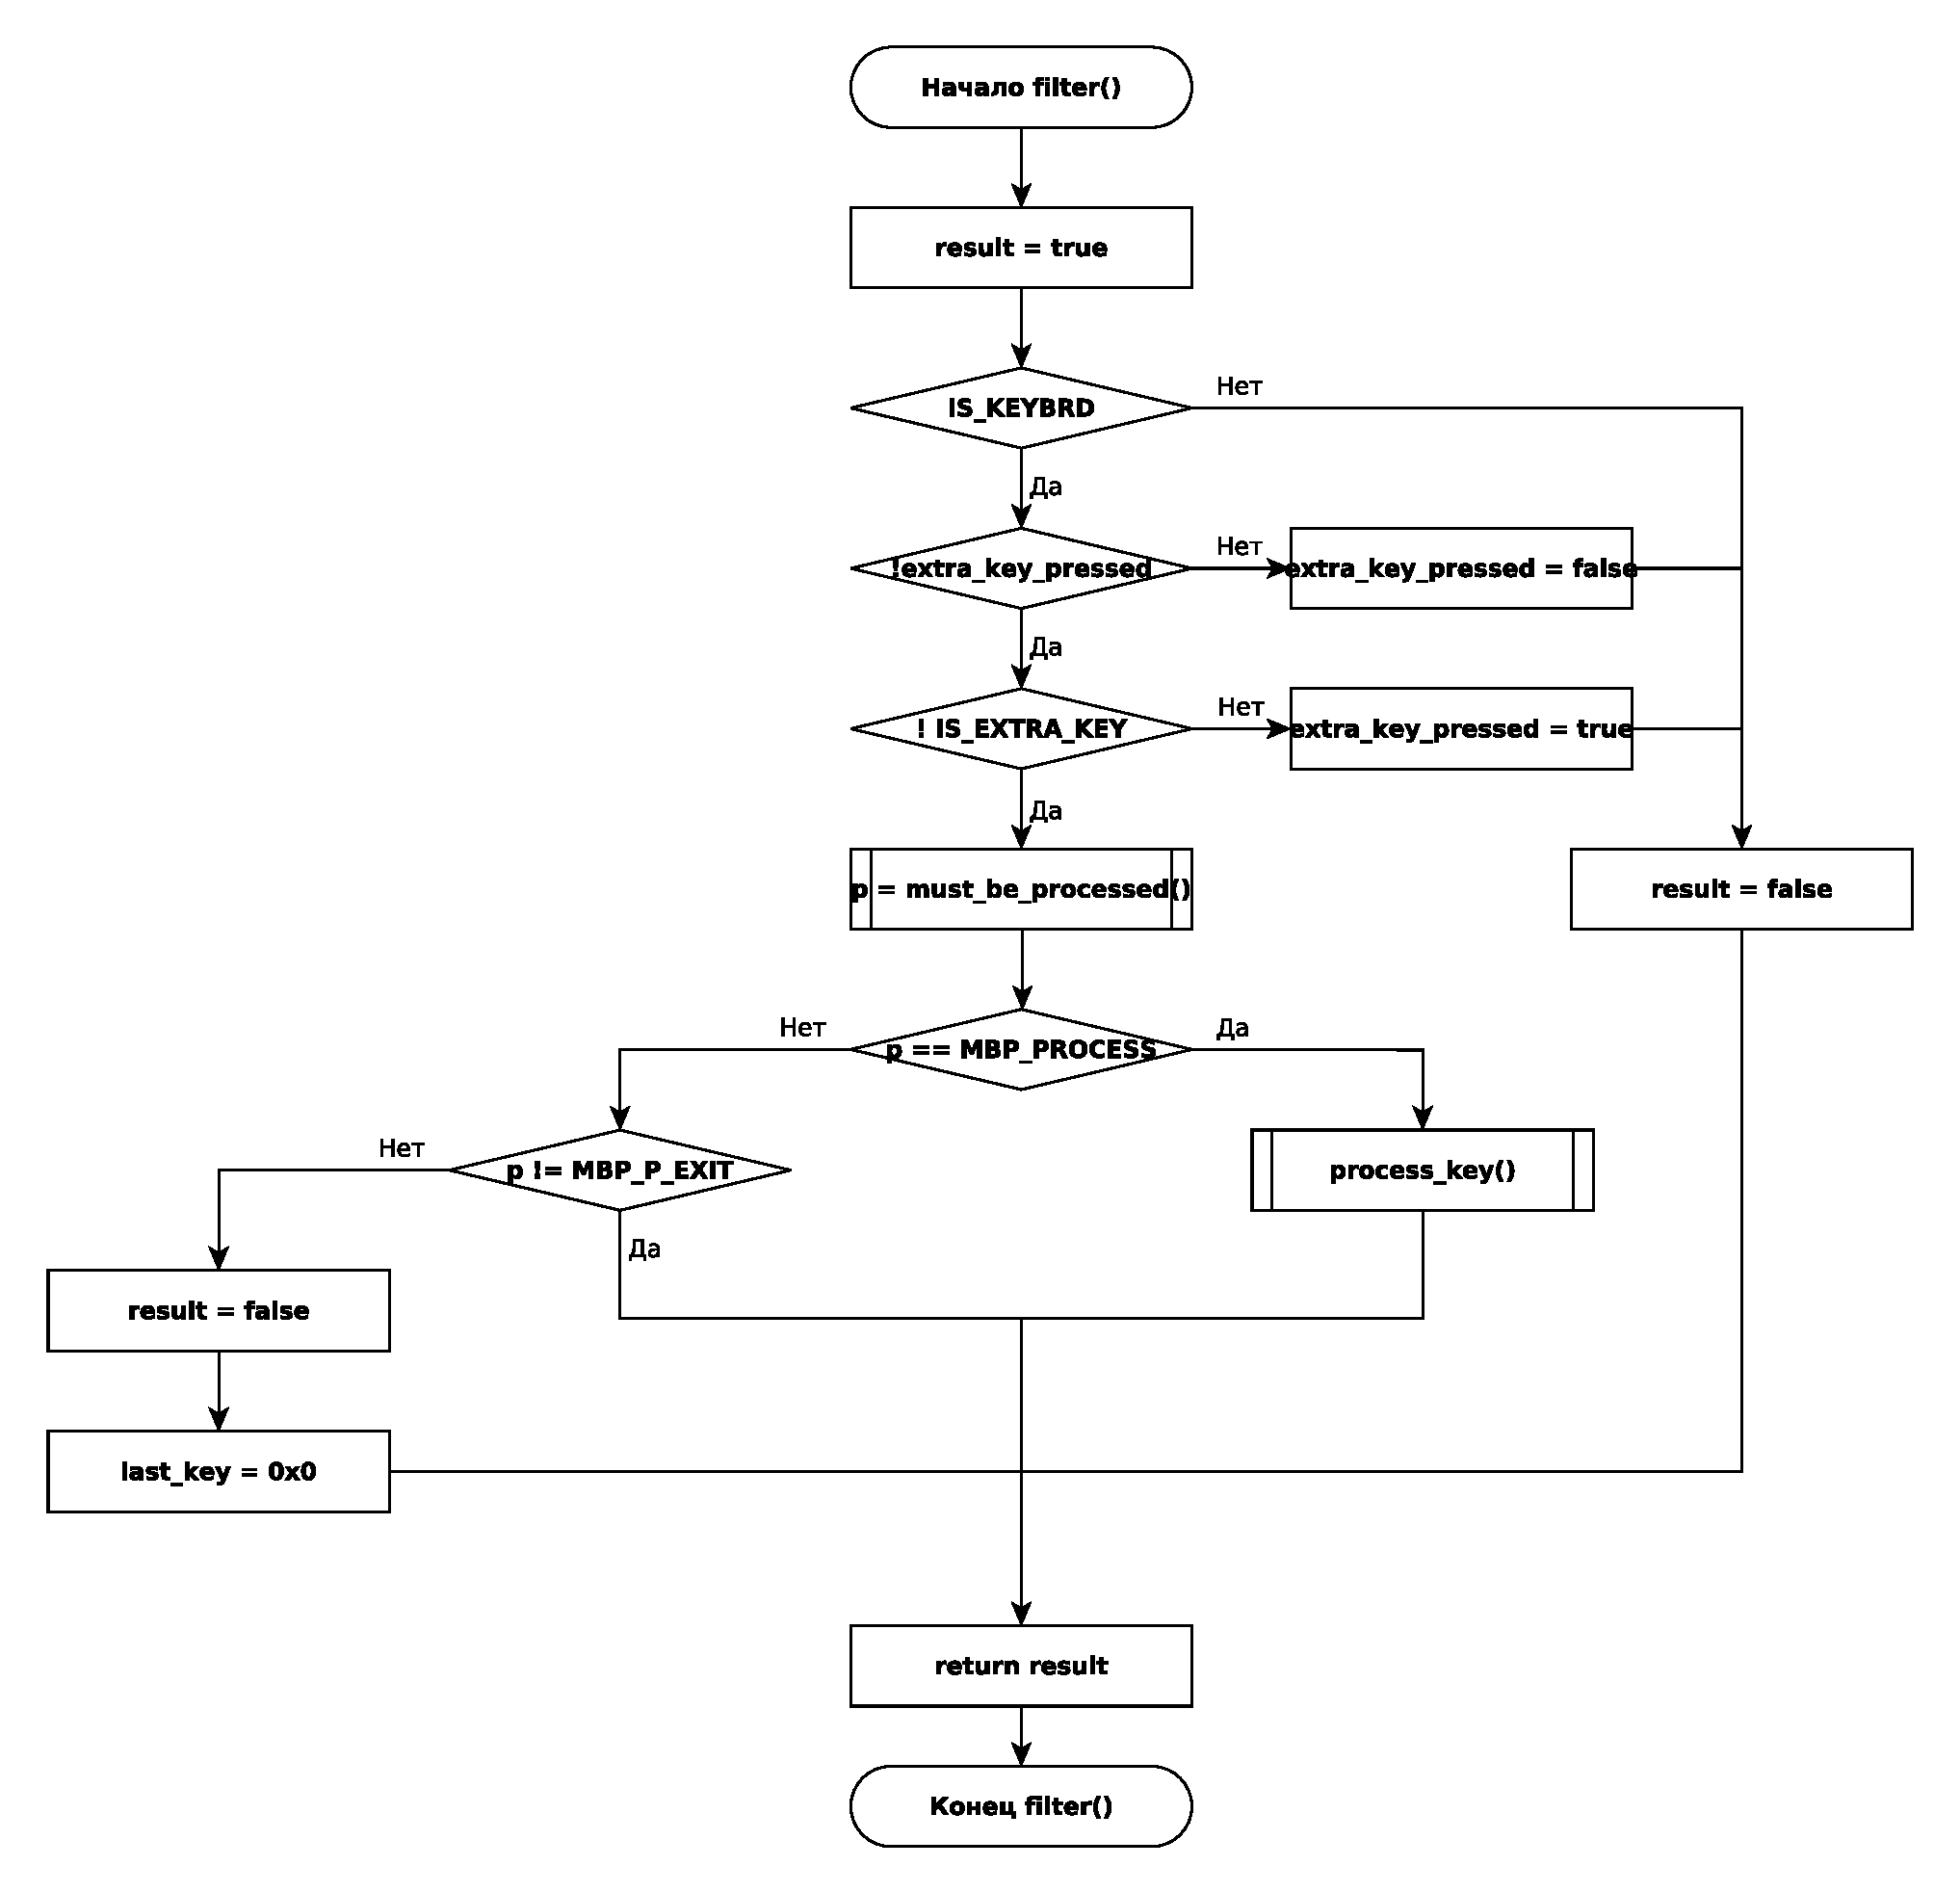
\includegraphics[scale=0.5]{filter.eps}
	\caption*{Алгоритм работы функции filter()}
\end{figure}
\begin{figure}[p]
	\centering
	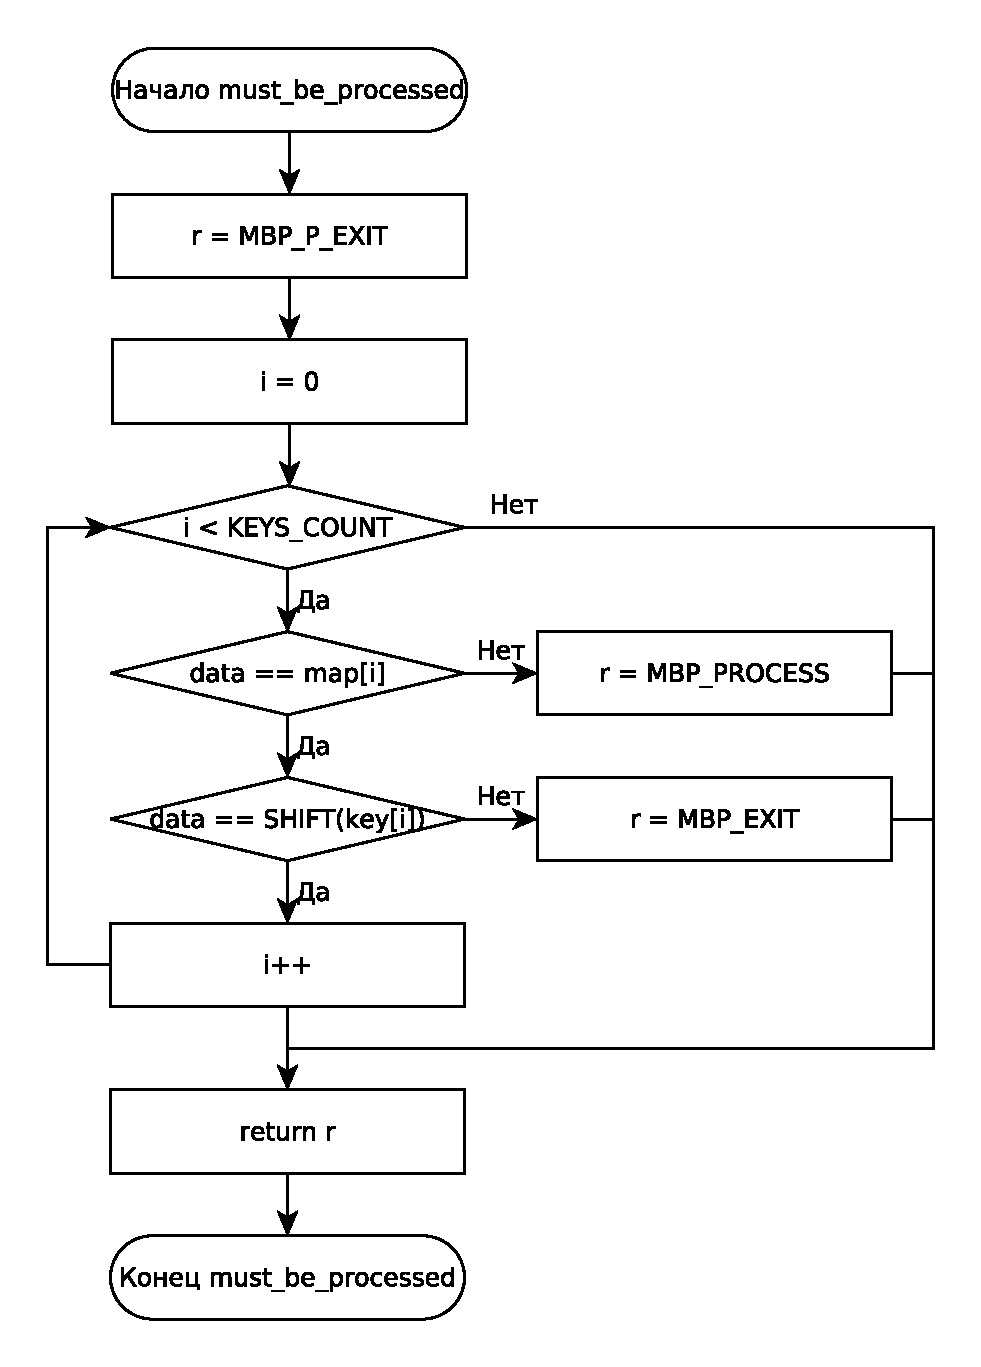
\includegraphics[scale=0.5]{must_be_processed.eps}
	\caption*{Алгоритм работы функции must\_be\_processed()}
\end{figure}
\newgeometry{top=1.5cm}
\begin{figure}[p]
	\centering
	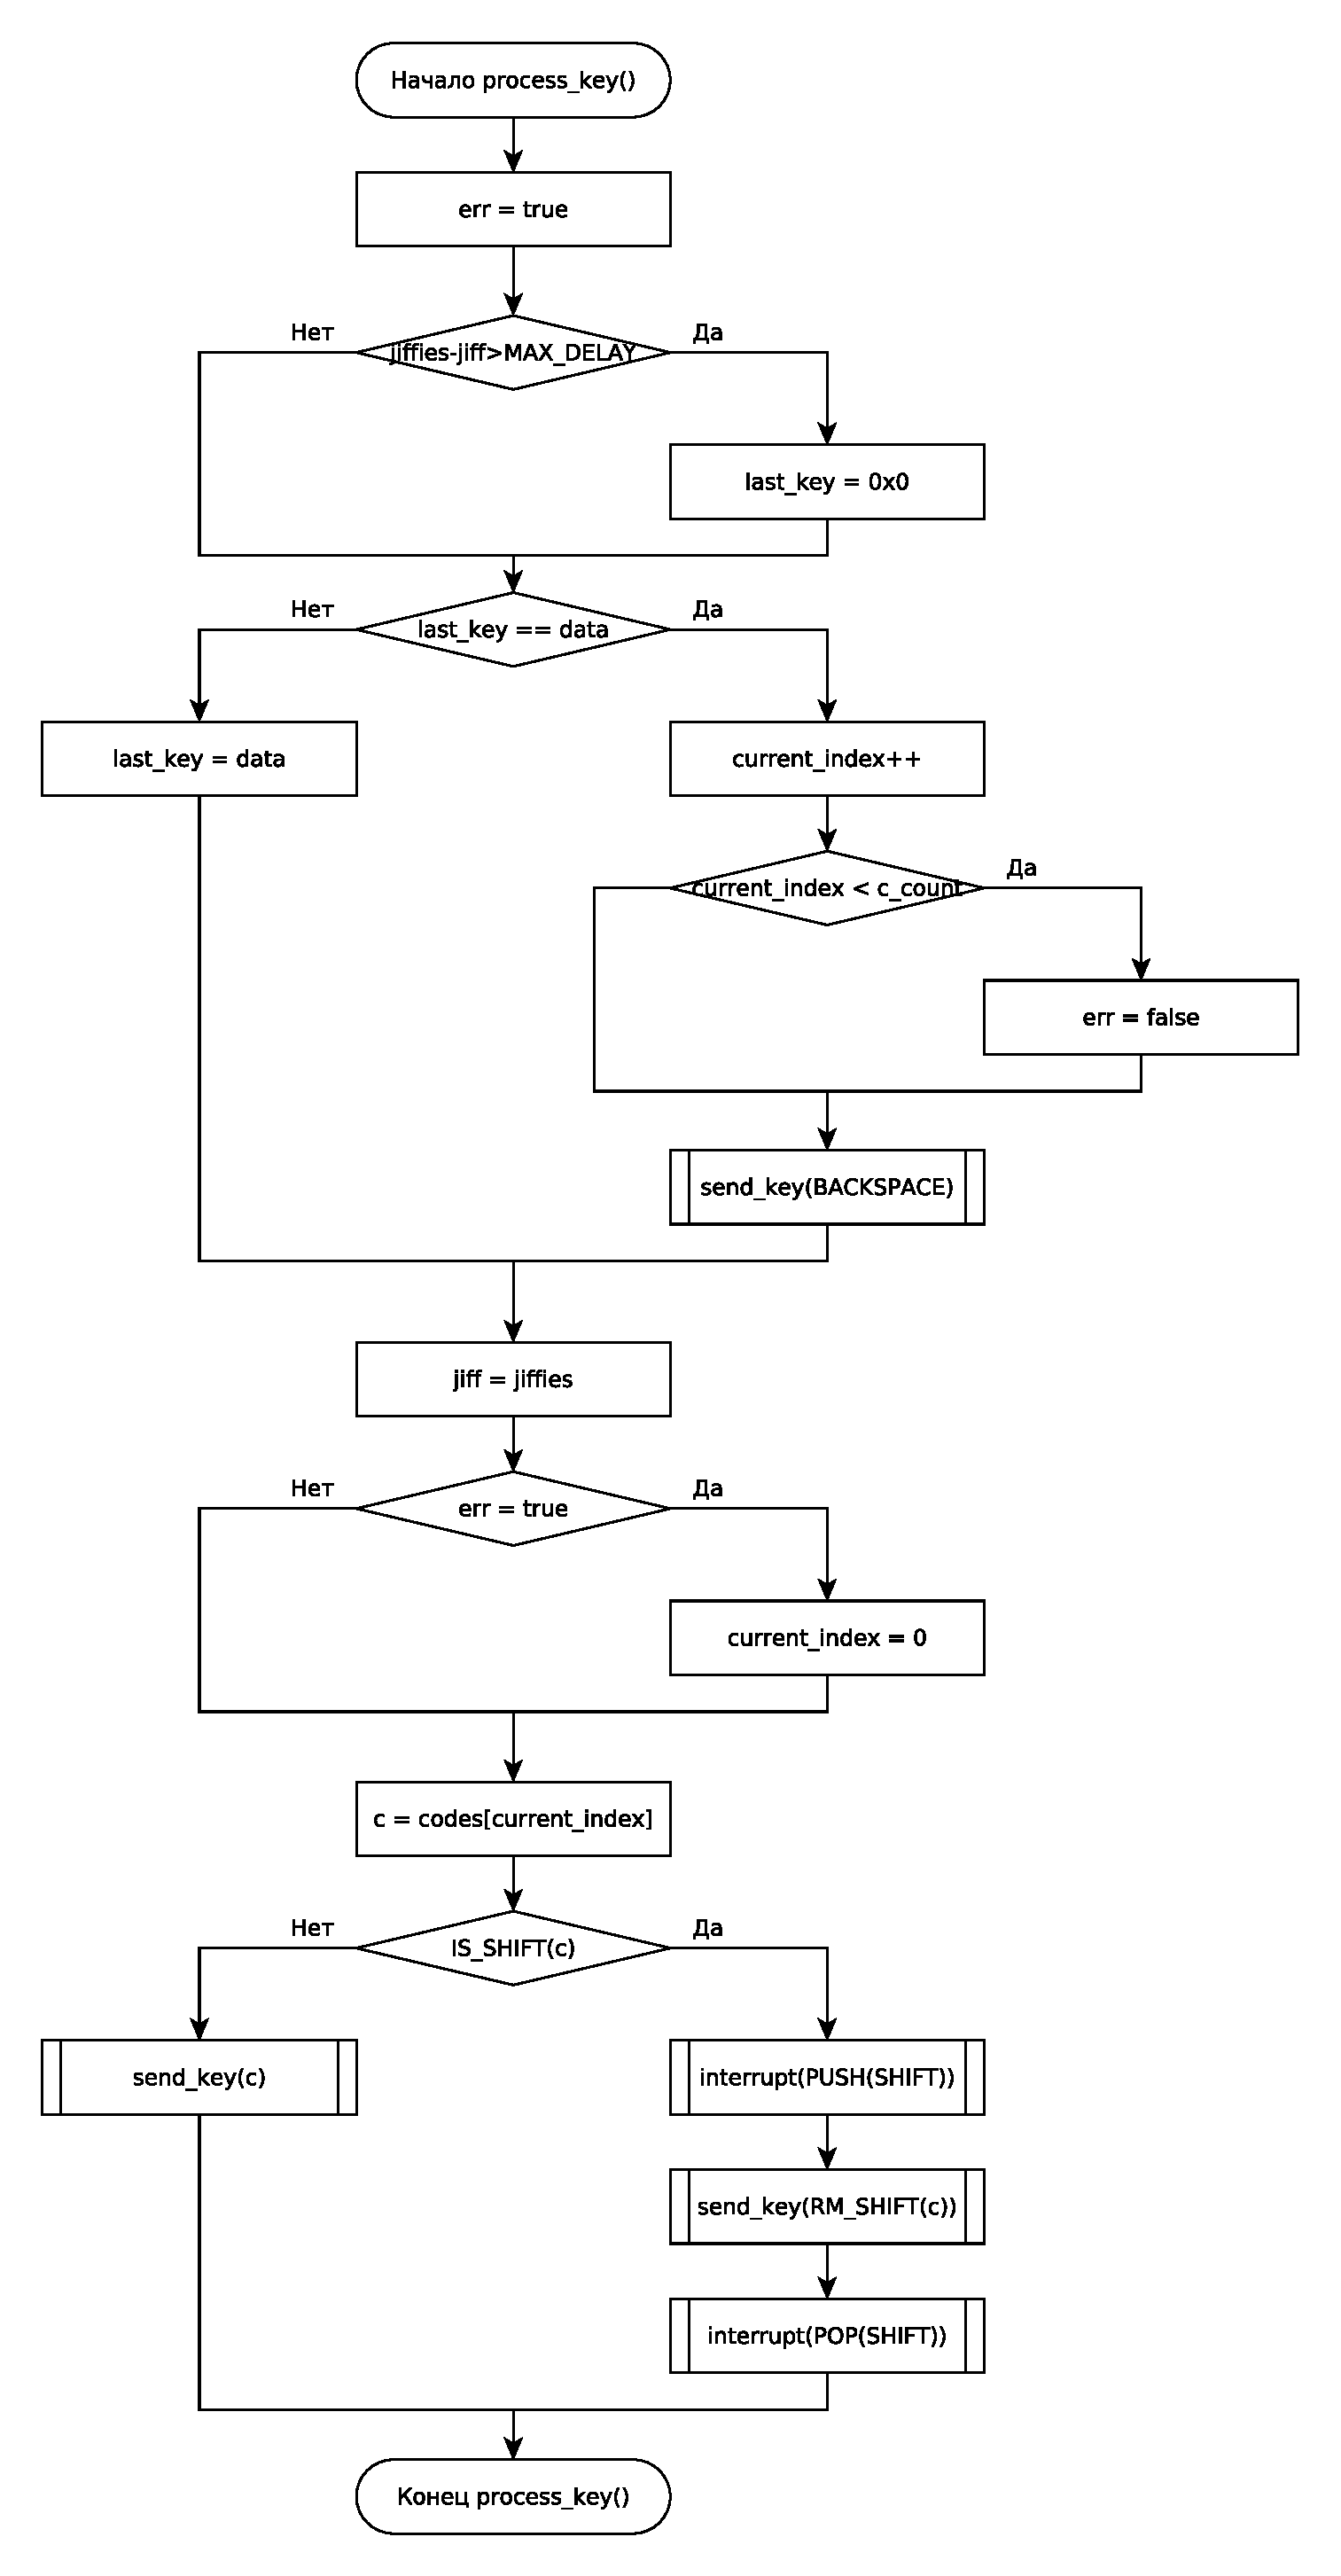
\includegraphics[scale=0.5]{process_key.eps}
	\caption*{Алгоритм работы функции process\_key()}
\end{figure}
\restoregeometry
\newpage

	\section{Технологический раздел}

\subsection{Среда разработки}
Для написания драйвера фильтра клавиатуры была выбрана операционная система \gnulinux.
Ядро данной операционной системы защищено лицензией GNU General Public License, согласно
которой его можно копировать, модифицировать и распространять.
\begin{flushleft}
	\begin{tabular}{ll}
		Операционная система:&\gnulinux\\
		Версия ядра:&\linuxv\\
		Дистрибутив:&\archlinux
	\end{tabular}
\end{flushleft}

\subsection{Выбор языка программирования}
Как и все <<уважающие себя>> ядра \unix, ядро \linux\ написано на языке \src{C}.
Но ядро \linux\ написано не на числом \src{C} в стандарте \src{ANSI C}. Где возможно,
разработчики ядра используют различные расширения языка, которые доступны
с помощью средств компиляции \src{gcc} (\src{GNU Compiler Collection}, где содержится
компилятор \src{C}, используемый для компиляции ядра).
\newpar
Разработчики ядра используют как расширения языка \src{C ISO C99}\footnote{Стандарт
\src{ISO C99}~--- последняя основная версия редакции стандарта \src{ISO C}.}, так и
расширения \src{GNU C}\ \cite{Love}.
\newpar
Поэтому, для написания модуля ядра был использован язык \src{C}.

\subsection{Среда программирования}
Разработка программного кода драйвера осуществлялась в текстовом редакторе \src{Vim}.
Ныне это один из мощнейших текстовых редакторов с полной свободой настройки 
и автоматизации, и созданным благодаря этому расширениям и надстройкам.

\newpar
Для компиляции исходного кода модуля была использована утилита \src{make}.
Данная утилита используя \src{Makefile} автоматизирует процесс компиляции и сборки
модуля ядра.
\newpar

Для отладки модуля была использована дополнительная виртуальная операционная система,
которая по своим параметрам полностью соответствует основной ОС, а именно:
\begin{flushleft}
	\begin{tabular}{ll}
		Операционная система:&\gnulinux\\
		Версия ядра:&\linuxv\\
		Дистрибутив:&\archlinux
	\end{tabular}
\end{flushleft}

\newpar
Отладочные сообщения позволяла просматривать утилита \src{dmesg} в сочетании с 
утилитой \src{grep}.

\subsection{Установка и использование программного обеспечения}
Для корректной работы программного обеспечения, его рекомендуется устанавливать
на систему с теми же характеристиками, которые были описаны выше. Однако установка
может так же производиться на операционные системы \gnulinux\ использующие ядро старше версии 
2.6.33\footnote{Именно в этой версии ядра были произведены последние изменения необходимых
для работы драйвера файлов.}. 
Так же для корректной генерации карты симполов необходимы библиотеки Python версии 3.3.2 или старше.
\newpar
Для компиляции проекта, неоходимо скопировать все модули проекта в текущую папку и запустить
утилиту \src{make}, предварительно отредактировав нужным образом переменную \src{KERNEL\_DIR} и,
при необходимости отладки, добавить в переменную \src{DEFINES} строку <<\src{DEBUG}>>.
\newpar

После успешной компиляции и сборки проекта в текущей директории появится файл \src{dFilter.ko}.
Для загрузки модуля в память, используйте команду \src{insmod dFilter.ko}, а для выгрузки~--
\src{rmmod dFilter}. В случае отладочной сборки, сообщения можно просматривать с помощью команды 
\src{dmesg | grep dFilter}\footnote{Для Вашего дистрибутива считывание сообщений может осуществляться иным образом.
	Если у Вас не установлена утилита \src{dmesg}, попробуйте считать лог-файл вручную: 
	\src{cat /var/log/messages | grep dFitler}.}.
\newpar

Для отображения текущей карты клавиш, необходимо выполнить команду
\src{./key\_codes.py}\footnote{Если расположение исполняемого файла \src{python} отлично от 
\linuxpath{/usr/bin/python}, попробуйте явно указать иной путь в shebang-строке скрипта или же явно передать скрипт на
выполнение установленной версии \src{python}.} предварительно выставив с помощью 
команды \src{chmod +x ./key\_codes.py} флаг выполнения для
файла \src{key\_codes.py}.
\newpar

Для изменения карты клавиш, отредактируйте файл \src{key\_map.conf}. Файл должен быть построен по следующим правилам:\\
\key{Код реальной клавиши} $->$ \key{Маска клавиш через пробел}\\
Маска клавиш указана в начале файла в блоке комментариев.
Комментарий начинается с символа \key{\#}. В случае, если в маске указан символ, который не был изначально предусмотрен
как часть маски или ключа, драйвер работать не будет. Внести коррективы в набор используемых
символов можно в файле \src{key\_codes.py} в переменной \src{key\_map}. Эта переменная представляет собой
словарь вида\\ \key{Символ} : \key{Скан-код символа}.
\newpar

Изменения в вышеуказанные файлы вводятся исключительно на стах и риск пользователя.
\newpage
\subsection{Исходные коды}
\subsubsection*{Заголовочный модуль \src{main\_header.h}}
\lstinputlisting[language = C, caption = {}]{../src/main_header.h}
\newpage
\subsubsection*{Модуль \src{main.c}}
\lstinputlisting[language = C, caption = {}]{../src/main.c}
\newpage
\subsubsection*{Заголовочный модуль \src{keyboard.h}}
\lstinputlisting[language = C, caption = {}]{../src/keyboard.h}
\newpage
\subsubsection*{Модуль \src{keyboard.c}}
\lstinputlisting[language = C, caption = {}]{../src/keyboard.c}
\newpage
\subsubsection*{Генерируемый заголовочный модуль \src{key\_map.h}}
\lstinputlisting[language = C, caption = {}]{../src/key_map.h}
\newpage
\subsubsection*{\src{Makefile}}
\lstinputlisting[caption = {}]{../Makefile}
\newpage
\subsubsection*{Скрипт \src{key\_codes.py}}
\lstinputlisting[language = Python, caption = {}]{../key_codes.py}
\newpage
\subsubsection*{Конфигурационный файл \src{key\_map.conf}}
\lstinputlisting[caption = {}]{../key_map.conf}
\newpage

	\addcontentsline{toc}{section}{Заключение}
\section*{Заключение}
Целью данной работы являлось исследование драйвера клавиатуры в ОС \linux\ и
написание драйвера-фильтра для изменения его поведения. Для реализации
поставленной задачи были изучены основные методы работы с ядром операционный
системы \gnulinux, а именно, были изучены и разобраны необходимые для
реализации поставленной задачи исходные коды ядра и был найден способ
благодаря которому удалось изменить стандартное поведение драйвера контроллера 
\src{i8042}.
\newpar
Поставленная задача была полностью реализована и протестирована.
Получившееся программное обеспечение удовлетворяет всем требованиям,
перечисленным при постановке задачи.
\newpage

%	\addcontentsline{toc}{section}{Приложение}
\section*{Приложение}

\newpage

	\newpage
	\addcontentsline{toc}{section}{\bibname}
	\nocite{*}
	\bibliography{biblio}
\end{document}
